\tikzset{every picture/.style={line width=0.75pt}} %set default line width to 0.75pt        

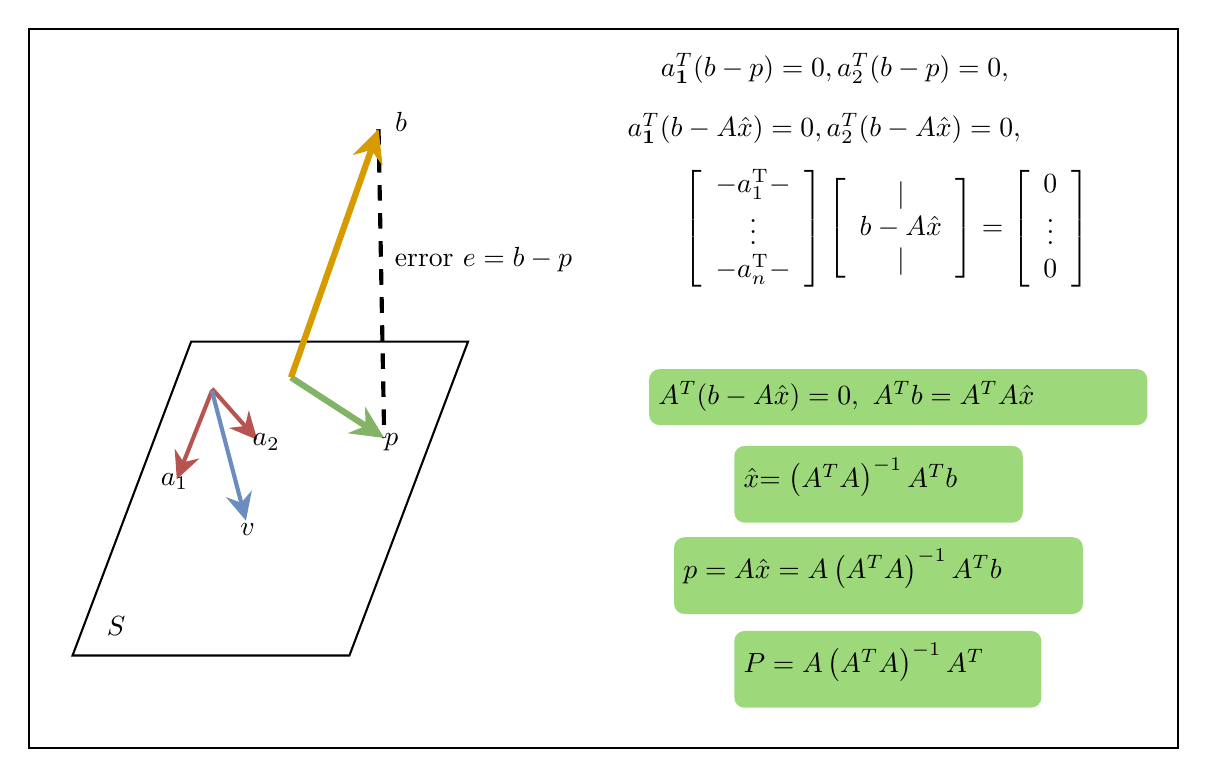
\begin{tikzpicture}[x=0.75pt,y=0.75pt,yscale=-1,xscale=1]
%uncomment if require: \path (0,350); %set diagram left start at 0, and has height of 350

%Straight Lines [id:da0833896477217686] 
\draw [color={rgb, 255:red, 130; green, 179; blue, 102 }  ,draw opacity=1 ][line width=2.25]    (127.38,169.03) -- (168.08,195.47) ;
\draw [shift={(172.28,198.19)}, rotate = 213] [fill={rgb, 255:red, 130; green, 179; blue, 102 }  ,fill opacity=1 ][line width=0.08]  [draw opacity=0] (16.07,-7.72) -- (0,0) -- (16.07,7.72) -- (10.67,0) -- cycle    ;
%Straight Lines [id:da7639150841734914] 
\draw [color={rgb, 255:red, 184; green, 84; blue, 80 }  ,draw opacity=1 ][line width=1.5]    (89.28,175.43) -- (73.82,214.38) ;
\draw [shift={(72.35,218.1)}, rotate = 291.64] [fill={rgb, 255:red, 184; green, 84; blue, 80 }  ,fill opacity=1 ][line width=0.08]  [draw opacity=0] (13.4,-6.43) -- (0,0) -- (13.4,6.44) -- (8.9,0) -- cycle    ;
%Straight Lines [id:da3617082286190523] 
\draw [line width=1.5]  [dash pattern={on 5.63pt off 4.5pt}]  (169.55,49.34) -- (172.28,198.19) ;
%Shape: Parallelogram [id:dp7592583426452624] 
\draw   (79.28,151.73) -- (212.68,151.73) -- (155.51,303) -- (22.11,303) -- cycle ;
%Straight Lines [id:da8449665178781662] 
\draw [color={rgb, 255:red, 184; green, 84; blue, 80 }  ,draw opacity=1 ][line width=1.5]    (89.28,174.43) -- (108.47,196.09) ;
\draw [shift={(111.12,199.08)}, rotate = 228.46] [fill={rgb, 255:red, 184; green, 84; blue, 80 }  ,fill opacity=1 ][line width=0.08]  [draw opacity=0] (13.4,-6.43) -- (0,0) -- (13.4,6.44) -- (8.9,0) -- cycle    ;
%Straight Lines [id:da21760172692551993] 
\draw [color={rgb, 255:red, 106; green, 140; blue, 190 }  ,draw opacity=1 ][line width=1.5]    (89.28,175.43) -- (104.64,234.14) ;
\draw [shift={(105.66,238.01)}, rotate = 255.32999999999998] [fill={rgb, 255:red, 106; green, 140; blue, 190 }  ,fill opacity=1 ][line width=0.08]  [draw opacity=0] (13.4,-6.43) -- (0,0) -- (13.4,6.44) -- (8.9,0) -- cycle    ;
%Straight Lines [id:da9743594112783229] 
\draw [color={rgb, 255:red, 215; green, 155; blue, 0 }  ,draw opacity=1 ][line width=2.25]    (127.38,169.03) -- (167.89,54.06) ;
\draw [shift={(169.55,49.34)}, rotate = 469.41] [fill={rgb, 255:red, 215; green, 155; blue, 0 }  ,fill opacity=1 ][line width=0.08]  [draw opacity=0] (16.07,-7.72) -- (0,0) -- (16.07,7.72) -- (10.67,0) -- cycle    ;
%Shape: Rectangle [id:dp3830905409317218] 
\draw   (1,1) -- (554.64,1) -- (554.64,347.62) -- (1,347.62) -- cycle ;

% Text Node
\draw (175.98,39.87) node [anchor=north west][inner sep=0.75pt]    {$\boldsymbol{b}$};
% Text Node
\draw (170.85,194.49) node [anchor=north west][inner sep=0.75pt]    {$\boldsymbol{p}$};
% Text Node
\draw (107.38,194.77) node [anchor=north west][inner sep=0.75pt]    {$\boldsymbol{a}_{2}$};
% Text Node
\draw (175.92,104.86) node [anchor=north west][inner sep=0.75pt]   [align=left] {error $\displaystyle \boldsymbol{e} =\boldsymbol{b-p}$};
% Text Node
\draw (63.21,213.92) node [anchor=north west][inner sep=0.75pt]    {$\boldsymbol{a}_{1}$};
% Text Node
\draw (101.48,237.88) node [anchor=north west][inner sep=0.75pt]    {$\boldsymbol{v}$};
% Text Node
\draw (37.18,282.9) node [anchor=north west][inner sep=0.75pt]    {$\boldsymbol{S}$};
% Text Node
\draw (288.11,40.4) node [anchor=north west][inner sep=0.75pt]    {$\boldsymbol{a}_{\mathbf{1}}^{T} (\boldsymbol{b} -\boldsymbol{A}\hat{\boldsymbol{x}} )=0,\boldsymbol{a}_{2}^{T} (\boldsymbol{b} -\boldsymbol{A}\hat{\boldsymbol{x}} )=0,\dotsc $};
% Text Node
\draw (304.11,11.4) node [anchor=north west][inner sep=0.75pt]    {$\boldsymbol{a}_{\mathbf{1}}^{T} (\boldsymbol{b} -\boldsymbol{p} )=0,\boldsymbol{a}_{2}^{T} (\boldsymbol{b} -\boldsymbol{p} )=0,\dotsc $};
% Text Node
\draw (314.93,67.4) node [anchor=north west][inner sep=0.75pt]    {$\left[\begin{array}{ c }
-\boldsymbol{a}_{1}^{\mathrm{T}} -\\
\vdots \\
-\boldsymbol{a}_{n}^{\mathrm{T}} -
\end{array}\right]\left[\begin{array}{ c }
\mid \\
\boldsymbol{b} -\boldsymbol{A\hat{\boldsymbol{x}}}\\
\mid 
\end{array}\right] =\left[\begin{array}{ c }
0\\
\vdots \\
0
\end{array}\right]$};
% Text Node
\draw  [color={rgb, 255:red, 0; green, 0; blue, 0 }  ,draw opacity=0 ][fill={rgb, 255:red, 157; green, 217; blue, 123 }  ,fill opacity=1 ]  (299.93,170) .. controls (299.93,167.24) and (302.17,165) .. (304.93,165) -- (534.93,165) .. controls (537.7,165) and (539.93,167.24) .. (539.93,170) -- (539.93,187) .. controls (539.93,189.76) and (537.7,192) .. (534.93,192) -- (304.93,192) .. controls (302.17,192) and (299.93,189.76) .. (299.93,187) -- cycle  ;
\draw (302.93,169.4) node [anchor=north west][inner sep=0.75pt]    {$\boldsymbol{A^{T} (b-A\hat{x} )} =0,\ \boldsymbol{A^{T} b=A^{T} A\hat{x}}$};
% Text Node
\draw  [color={rgb, 255:red, 0; green, 0; blue, 0 }  ,draw opacity=0 ][fill={rgb, 255:red, 157; green, 217; blue, 123 }  ,fill opacity=1 ]  (340.93,207) .. controls (340.93,204.24) and (343.17,202) .. (345.93,202) -- (474.93,202) .. controls (477.7,202) and (479.93,204.24) .. (479.93,207) -- (479.93,234) .. controls (479.93,236.76) and (477.7,239) .. (474.93,239) -- (345.93,239) .. controls (343.17,239) and (340.93,236.76) .. (340.93,234) -- cycle  ;
\draw (343.93,206.4) node [anchor=north west][inner sep=0.75pt]    {$\hat{\boldsymbol{x}}\boldsymbol{=\left( A^{T} A\right)^{-1} A^{T} b}$};
% Text Node
\draw  [color={rgb, 255:red, 157; green, 217; blue, 123 }  ,draw opacity=0 ][fill={rgb, 255:red, 157; green, 217; blue, 123 }  ,fill opacity=1 ]  (311.93,251) .. controls (311.93,248.24) and (314.17,246) .. (316.93,246) -- (503.93,246) .. controls (506.7,246) and (508.93,248.24) .. (508.93,251) -- (508.93,278) .. controls (508.93,280.76) and (506.7,283) .. (503.93,283) -- (316.93,283) .. controls (314.17,283) and (311.93,280.76) .. (311.93,278) -- cycle  ;
\draw (314.93,250.4) node [anchor=north west][inner sep=0.75pt]    {$\boldsymbol{p=A\hat{x} =A\left( A^{T} A\right)^{-1} A^{T} b}$};
% Text Node
\draw  [color={rgb, 255:red, 0; green, 0; blue, 0 }  ,draw opacity=0 ][fill={rgb, 255:red, 157; green, 217; blue, 123 }  ,fill opacity=1 ]  (340.93,296.15) .. controls (340.93,293.38) and (343.17,291.15) .. (345.93,291.15) -- (483.93,291.15) .. controls (486.7,291.15) and (488.93,293.38) .. (488.93,296.15) -- (488.93,323.15) .. controls (488.93,325.91) and (486.7,328.15) .. (483.93,328.15) -- (345.93,328.15) .. controls (343.17,328.15) and (340.93,325.91) .. (340.93,323.15) -- cycle  ;
\draw (343.93,295.55) node [anchor=north west][inner sep=0.75pt]    {$\boldsymbol{P=A\left( A^{T} A\right)^{-1} A^{T}}$};


\end{tikzpicture}
